



\documentclass[a4paper,12pt,spanish]{article}

\usepackage[utf8]{inputenc}


\usepackage{blindtext}
%\usepackage{microtype}
\usepackage{amsfonts, amsmath, amsthm, amssymb}
%\usepackage{fancyhdr}
%\usepackage{index}
%\usepackage{multicol}    

%\usepackage{booktabs}

\usepackage[T1]{fontenc}
\usepackage[utf8]{inputenc}
\usepackage{graphicx}
\usepackage[spanish,es-tabla]{babel}
\usepackage{url}
\usepackage{enumitem}

\usepackage[unicode=true, pdfusetitle,
bookmarks=true,bookmarksnumbered=false,bookmarksopen=false,
breaklinks=true,pdfborder={0 0 1},backref=false,colorlinks=false]
{hyperref}

\usepackage{listings}
\usepackage{longtable}


\usepackage{siunitx} %para el sistema internacional
\usepackage[export]{adjustbox}
\usepackage{booktabs} 
\usepackage{subcaption}

\usepackage{float}


\newcommand{\address}[1]{
	\par {\raggedright #1
		\vspace{1.4em}
		\noindent\par}
}

\usepackage[table,xcdraw]{xcolor}


\pagenumbering{gobble}
\include{noNumberPage}
\pagenumbering{arabic}
\setcounter{page}{14}

%tutorial de tablas latex: https://manualdelatex.com/tutoriales/tablas

\usepackage{multirow}

% \usepackage[table,xcdraw]{xcolor}


%Inicio del documento (hasta que se cierre con \end{document}
\begin{document}
	
	
	\title{Ecuación de estado y Punto crítico}
	
	%\author{Adrián Rivero Fernández}
	\date{}
	
	\maketitle
	
	
	\iffalse %comentarios de varias líneas con un if, poner en true si queremos que suceda
	\begin{abstract} %resumen
		
		
		Pretendemos estudiar la conservación de la energía mecánica de un sólido con rotación y desplazamiento, y la determinación del momento de inercia de la rueda de Maxwell.
		
		
		
	\end{abstract} 
	\fi
	
\iffalse
I don't want this to happen
\fi



	
	\section{Objetivos de la práctica}
	
	
	\begin{enumerate}
		\item Obtener los valores ($P$, $V$) para la representación gráfica de las isotermas de
		un gas (etano) tanto para la región de gas puro como para la región de coexistencia de fases gas-líquido (isotermas de Andrews).
		\item Describir el comportamiento de un gas real (etano), que no verifica la
		ecuación de estado de los gases ideales, por medio de la ecuación de Van der
		Waals. Determinar de los parámetros $a$, $b$ de dicha ecuación así como el
		número de moles de una muestra de etano
		\item Estimar el punto crítico y determinar las constantes críticas del sistema.
		\item Obtener experimentalmente la curva de presión de vapor del gas y del calor latente
	\end{enumerate}
	
	
	
	
	\section{Resumen teórico}
	
	
	
	La ecuación de Van der Waals para el gas real
	\[\left(P + \frac{a}{V_m^2}\right)(V_m - b) = RT
	\]
	cuando $a \rightarrow 0$  y $b \rightarrow 0$ se reduce a la ecuación del gas ideal
	\[PV_m = RT\]
	


	Las fases de un sistema puro se representan en un diagrama $P - V_m$ en función de la presión y el volumen molar, como en la figura \ref{fig:diagrama}
	
	\begin{figure}[H]
		\centering
		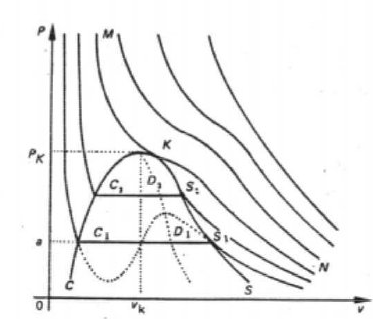
\includegraphics[width=0.5\linewidth]{imagenes/image.6OCH31}
		\caption{diagrama de fases}
		\label{fig:diagrama}
	\end{figure}
	
	
	Podemos distinguir en ella el punto crítico $K$, en el punto más alto de la campana, que separa la región de fase líquida, a la izquierda de la rama $CK$, de la fase gaseosa, a la derecha de la rama $KS$, y de la zona de coexistencia, bajo la curva $cKS$.
	La isoterma crítica $MN$ separa la región del diagrama en la que el gas puede licuarse o no por una compresión a temperatura constante. 
	En la zona de coexistencia las isotermas son paralelas al eje de abscisas, de modo que variando el volumen se obtiene un cambio de fase sin variar la presión de equilibrio. En este caso el módulo de compresibilidad isoterma del gas diverge:
	\[ \frac{1}{k_T} = -\frac{1}{V_m} \left(\frac{\partial V_m}{\partial P}\right)_T \rightarrow \infty
 	\]
	La aproximación del gas ideal deja de ser válida en cada isoterma al aproximarse a la campana de coexistencia. Aquí toma importancia el modelo de campo medio, que da lugar a la ecuación de Van der Waals, y describe correctamente la isoterma cerca de la zona de coexistencia, cuando la interacción entre las moléculas comienza a ser importante.
	
	
	\subsection*{Transición de fase (de primer orden)}
	
	
	Cuando en un recinto aislado existe una mezcla de dos fases del mismo componente, la transición de fase es un proceso reversible y abierto para cada una de las fases, de modo que hay posibilidad de intercambio de partículas entre las fases. Por ello la variación de energía y entropía del sistema satisface 
	\[ dU = 0 = dU_1 + dU_2
	\]
	\[ dS = 0 = dS_1 + dS_2
	\]
	
	para cada uno de los sistemas abiertos
	\[ T_i dS_i = dU_i + P_i dV_i - \mu_i dN_i	\]
	
	siendo $S= S(U,N,V)$ y $\mu$ el potencialh químico (energía libre de Gibbs). Como $dV_1= -dV_2$, $dN_2 = - dN_1$, $dU_1= - dU_2$, la condición de equilibrio termodinámico entre las dos fases en el punto de transición es el conjunto de igualdades de presión, temperatura y potencial químico:
	\[T_1= T_2\]
	\[ P_1= P_2\]
	\[\mu_1= \mu_2\]
	
	Los cambios de fase se denominan de primer orden porque la s derivadas primeras de la energía específica $g$ de Gibbs (o potencial quimico $\mu$)
	\[G=U-TS+PV\]
	\[ g = \frac{G}{n}\rightarrow dg = -sdT + V_m dP
	\]
	son discontinuas en el punto de transición, lo que implica que sus valores para la fase líquido y fase vapor son diferentes. Para este caso las funciones discontinuas serán la entropía específica $s$ y el volumen molar $V_m$.
	
	\subsection*{Ecuación de Clausius-Clapeyron}
	
	La condición de equilibrio termodinámico se escribe
	\[g_1= g_2 \rightarrow dg_1 = dg_2 
	\]
	
	La energía necesaria para llevar una partícula de la fase 1 a la fase 2 es la misma que para llevarla de la fase 2 a la fase 1. En función de la temperatura y la presión del equilibrio
	\[T= T_1=T_2 \]
	\[ P= P_1=P_2
	\]
	obtenemos la relación
	\[-s_1 dT+V_{m1}dP= -s_2 dT+ V_{m2}dP\]
	podemos despejar la derivada
	\[\frac{dP}{dT}= \frac{s_2-s_1}{V_{m2}-V_{m1}}
	\]
	
	Para la transición líquido-vapor, la presión $P$ recibe el nombre de \textit{presión de vapor}. Como $s_2-s_1$ en un proceso reversible es el incremento de entropía del sistema por partícula, al transicionar de la fase 1 a la 2
	\[s_2-s_1 = \frac{Q_{12}}{T}= \frac{\mathcal{L}}{T}
	\]
	
	siendo $\mathcal{L}$ la energía necesaria para esa transformación, o \textit{calor latente} para la transición de fase. La relación anterior es por tanto 
	\[\frac{dP}{dT} = \frac{\mathcal{L}}{T\cdot \Delta V_m}
	\]
	
	que se conoce como la \textit{ecuación de Clausius-Clapeyron}, y se cumple a lo largo de la curva de equilibrio de coexistencia de ambas fases.
	
	En el caso de la vaporización, lejos de la temperatura crítuca, el volumen molar del gas es mucho mayor que el volumen molar del líquido, $V_{m2}>> V_{m1}$. Esto permite la aproximación
	\[\frac{dP}{dT} \approx \frac{\mathcal{L}}{T\cdot V_{m2}}
	\]
	Suponiendo que el gas se comporta de forma casi ideal, $V_{m2} = RT/P$, y la ecuación resultante se puede integrar,
	\[\frac{1}{P} \frac{dP}{dT} \approx \frac{\mathcal{L}}{RT^2} \rightarrow \ln P = -\frac{\mathcal{L}}{RT} + \text{cte}
	\]
	obteniendo la \textit{ecuación integrada de Clausius-Clapeyron}, que puede aplicarse a las medidas de presión de vapor frente a la temperatura pese a las aproximaciones realizadas.
	
	
	
	\section{Procedimiento experimental.}
	
	El dispositivo experimental se compone de un cilindro de vvidriograduado en mililitros. Su extremo inferior está sellado por una columna de mercurio, y en su interior se encuentra etano confinado.\\
	
	La columna de mercurio funciona como un pistón reduciendo o aumentando el volumen del gas en el cilindro según el sentido en el que accionemos el volante de presión. Un manómetro graduado en pascales indica la presión del interior de la columna de vidrio. El cilindro está alojado en una cubierta cilíndrica de metacrilato por donde circula agua procedente de un baño termostático. La temperatura de este agua se mide con un termómetro incrustado en la cubierta de metacrilato. Con este sistema podemos medir la temperatura y mantenerla constante mientras variamos la presión y el volumen, de modo que podamos obtener la isoterma.\\
	
	Durante las mediciones, hay que tener cuidado de no sobrepasar los $50\cdot 10^5 \si{Pa}$, ya que a superiores presiones existe riesgo de rotura del cilindro de vidrio. También conviene esperar a que el gas y el mercurio se equilibren a cada presión consignada, teniendo cada vez más cuidado cuanto más nos aproximamos a la región de coexistencia de fases.\\
	
	Tomaremos medidas para cinco isotermas, correspondientes a distintas temperaturas, distribuidas por encima y por debajo de la temperatura crítica.\\
	
	En el punto en el que cada isoterma cruza la campana de coexistencia podremos observar como se forma una capa de liquido sobre la columna del mercurio, y que la presión del manómetro se mantiene constante al reducir el volumen. Llegará un punto en que la capa de líquido aumenta hasta solo existir fase líquida, en ese punto se alcanza el extremo de la campana de coexistencia, y al tener los líquidos una baja compresibilidad, reducir más el volumen incrementaría enormemente la presión.\\
	
	Para cada isoterma de Andrews tomaremos los valores extremos de volumen en la región de coexistencia, para la fase gas $V_G$ y para la fase líquida $V_L$. Con ellos y conocido el número de moles de gas en el sistema, $n$, se podrán determinar los volúmenes molares de ambas fases a la temperatura dada
	
	\[ V_{mG} = \frac{V_G}{n} 
	\]
	\[V_{mL} = \frac{V_L}{n} \]
	
	son los valores característicos de la transición para una isoterma.\\
	
	Para la temperatura crítica el tramo rectilíneo de coexistencia en el diagrama se reduce a un único punto, y ambos volúmenes molares coinciden.
	
	
	\section{Tablas de medidas.}
	
	\begin{longtable}[c]{c|ccccc|}
		%\centering
		%\begin{tabular}{c|ccccc|}
			\cline{2-6}
			& \multicolumn{1}{c|}{\begin{tabular}[c]{@{}c@{}}T=21,1\\ $(\pm 0,1) \text{ºC}$\end{tabular}} & \multicolumn{1}{c|}{\begin{tabular}[c]{@{}c@{}}T=10,0 \\ $(\pm 0,1) \text{ºC}$\end{tabular}} & \multicolumn{1}{c|}{\begin{tabular}[c]{@{}c@{}}T=15\\ $(\pm 0,1) \text{ºC}$\end{tabular}} & \multicolumn{1}{c|}{\begin{tabular}[c]{@{}c@{}}T=25\\ $(\pm 0,1) \text{ºC}$\end{tabular}} & \begin{tabular}[c]{@{}c@{}}T=30\\ $(\pm 0,1) \text{ºC}$\end{tabular} \\ \hline
			\multicolumn{1}{|c|}{V $(\pm 0,05)\si{ml}$}  & \multicolumn{5}{c|}{Presion $(\pm 0,5) \si{Pa\cdot 10^5}$}                                                                                           \\ \hline%\hline
			\multicolumn{1}{|c|}{3,90} & \multicolumn{1}{c|}{10,5}   & \multicolumn{1}{c|}{10,5} & \multicolumn{1}{c|}{10,5} & \multicolumn{1}{c|}{10,5} & 11,0 \\ \hline
			\multicolumn{1}{|c|}{3,80} & \multicolumn{1}{c|}{11,0}   & \multicolumn{1}{c|}{10,5} & \multicolumn{1}{c|}{10,5} & \multicolumn{1}{c|}{11,0} & 11,5 \\ \hline
			\multicolumn{1}{|c|}{3,70} & \multicolumn{1}{c|}{11,0}   & \multicolumn{1}{c|}{10,5} & \multicolumn{1}{c|}{11,0} & \multicolumn{1}{c|}{11,0} & 11,5 \\ \hline
			\multicolumn{1}{|c|}{3,60} & \multicolumn{1}{c|}{11,5}   & \multicolumn{1}{c|}{11,0} & \multicolumn{1}{c|}{11,0} & \multicolumn{1}{c|}{11,5} & 12,0 \\ \hline
			\multicolumn{1}{|c|}{3,50} & \multicolumn{1}{c|}{12,0}   & \multicolumn{1}{c|}{11,0} & \multicolumn{1}{c|}{11,5} & \multicolumn{1}{c|}{12,0} & 12,0 \\ \hline
			\multicolumn{1}{|c|}{3,40} & \multicolumn{1}{c|}{12,0}   & \multicolumn{1}{c|}{11,5} & \multicolumn{1}{c|}{12,0} & \multicolumn{1}{c|}{12,0} & 12,5 \\ \hline
			\multicolumn{1}{|c|}{3,30} & \multicolumn{1}{c|}{12,5}   & \multicolumn{1}{c|}{12,0} & \multicolumn{1}{c|}{12,0} & \multicolumn{1}{c|}{12,5} & 13,0 \\ \hline
			\multicolumn{1}{|c|}{3,20} & \multicolumn{1}{c|}{13,0}   & \multicolumn{1}{c|}{12,0} & \multicolumn{1}{c|}{12,5} & \multicolumn{1}{c|}{13,0} & 13,0 \\ \hline
			\multicolumn{1}{|c|}{3,10} & \multicolumn{1}{c|}{13,5}   & \multicolumn{1}{c|}{12,5} & \multicolumn{1}{c|}{13,0} & \multicolumn{1}{c|}{13,5} & 13,5 \\ \hline
			\multicolumn{1}{|c|}{3,00} & \multicolumn{1}{c|}{13,5}   & \multicolumn{1}{c|}{13,0} & \multicolumn{1}{c|}{13,5} & \multicolumn{1}{c|}{14,0} & 14,0 \\ \hline
			\multicolumn{1}{|c|}{2,90} & \multicolumn{1}{c|}{14,0}   & \multicolumn{1}{c|}{13,5} & \multicolumn{1}{c|}{14,0} & \multicolumn{1}{c|}{14,0} & 14,4 \\ \hline
			\multicolumn{1}{|c|}{2,80} & \multicolumn{1}{c|}{14,5}   & \multicolumn{1}{c|}{14,0} & \multicolumn{1}{c|}{14,0} & \multicolumn{1}{c|}{14,5} & 15,0 \\ \hline
			\multicolumn{1}{|c|}{2,70} & \multicolumn{1}{c|}{15,0}   & \multicolumn{1}{c|}{14,5} & \multicolumn{1}{c|}{14,5} & \multicolumn{1}{c|}{15,0} & 15,5 \\ \hline
			\multicolumn{1}{|c|}{2,60} & \multicolumn{1}{c|}{15,5}   & \multicolumn{1}{c|}{15,0} & \multicolumn{1}{c|}{15,0} & \multicolumn{1}{c|}{15,5} & 16,0 \\ \hline
			\multicolumn{1}{|c|}{2,50} & \multicolumn{1}{c|}{16,0}   & \multicolumn{1}{c|}{15,5} & \multicolumn{1}{c|}{15,5} & \multicolumn{1}{c|}{16,0} & 16,5 \\ \hline
			\multicolumn{1}{|c|}{2,40} & \multicolumn{1}{c|}{16,5}   & \multicolumn{1}{c|}{16,0} & \multicolumn{1}{c|}{16,0} & \multicolumn{1}{c|}{17,0} & 17,5 \\ \hline
			\multicolumn{1}{|c|}{2,30} & \multicolumn{1}{c|}{17,5}   & \multicolumn{1}{c|}{16,5} & \multicolumn{1}{c|}{17,0} & \multicolumn{1}{c|}{17,5} & 18,0 \\ \hline
			\multicolumn{1}{|c|}{2,20} & \multicolumn{1}{c|}{18,0}   & \multicolumn{1}{c|}{17,0} & \multicolumn{1}{c|}{17,5} & \multicolumn{1}{c|}{18,5} & 18,5 \\ \hline
			\multicolumn{1}{|c|}{2,10} & \multicolumn{1}{c|}{19,5}   & \multicolumn{1}{c|}{18,0} & \multicolumn{1}{c|}{18,5} & \multicolumn{1}{c|}{19,0} & 19,5 \\ \hline
			\multicolumn{1}{|c|}{2,00} & \multicolumn{1}{c|}{19,5}   & \multicolumn{1}{c|}{18,5} & \multicolumn{1}{c|}{19,0} & \multicolumn{1}{c|}{20,0} & 20,0 \\ \hline
			\multicolumn{1}{|c|}{1,90} & \multicolumn{1}{c|}{20,5}   & \multicolumn{1}{c|}{19,5} & \multicolumn{1}{c|}{20,0} & \multicolumn{1}{c|}{20,5} & 21,5 \\ \hline
			\multicolumn{1}{|c|}{1,80} & \multicolumn{1}{c|}{21,5}   & \multicolumn{1}{c|}{20,0} & \multicolumn{1}{c|}{21,0} & \multicolumn{1}{c|}{21,5} & 22,5 \\ \hline
			\multicolumn{1}{|c|}{1,70} & \multicolumn{1}{c|}{22,5}   & \multicolumn{1}{c|}{21,0} & \multicolumn{1}{c|}{22,0} & \multicolumn{1}{c|}{23,0} & 23,5 \\ \hline
			\multicolumn{1}{|c|}{1,60} & \multicolumn{1}{c|}{23,5}   & \multicolumn{1}{c|}{22,0} & \multicolumn{1}{c|}{23,0} & \multicolumn{1}{c|}{24,0} & 24,5 \\ \hline
			\multicolumn{1}{|c|}{1,50} & \multicolumn{1}{c|}{24,5}   & \multicolumn{1}{c|}{23,0} & \multicolumn{1}{c|}{24,0} & \multicolumn{1}{c|}{25,5} & 26,0 \\ \hline
			\multicolumn{1}{|c|}{1,40} & \multicolumn{1}{c|}{26,0}   & \multicolumn{1}{c|}{24,5} & \multicolumn{1}{c|}{25,0} & \multicolumn{1}{c|}{27,0} & 27,5 \\ \hline
			\multicolumn{1}{|c|}{1,30} & \multicolumn{1}{c|}{27,5}   & \multicolumn{1}{c|}{26,0} & \multicolumn{1}{c|}{27,0} & \multicolumn{1}{c|}{28,5} & 29,0 \\ \hline
			\multicolumn{1}{|c|}{1,20} & \multicolumn{1}{c|}{29,5}   & \multicolumn{1}{c|}{27,5} & \multicolumn{1}{c|}{28,5} & \multicolumn{1}{c|}{30,0} & 31,0 \\ \hline
			\multicolumn{1}{|c|}{1,10} & \multicolumn{1}{c|}{31,5}   & \multicolumn{1}{c|}{29,0} & \multicolumn{1}{c|}{30,0} & \multicolumn{1}{c|}{32,0} & 33,0 \\ \hline
			\multicolumn{1}{|c|}{1,00} & \multicolumn{1}{c|}{33,0}   & \multicolumn{1}{c|}{30,5} & \multicolumn{1}{c|}{32,0} & \multicolumn{1}{c|}{34,5} & 35,5 \\ \hline
			\multicolumn{1}{|c|}{0,90} & \multicolumn{1}{c|}{35,0}   & \multicolumn{1}{c|}{31,5} & \multicolumn{1}{c|}{33,5} & \multicolumn{1}{c|}{36,5} & 37,5 \\ \hline
			\multicolumn{1}{|c|}{0,80} & \multicolumn{1}{c|}{37,5}   & \multicolumn{1}{c|}{31,5} & \multicolumn{1}{c|}{35,5} & \multicolumn{1}{c|}{39,0} & 40,5 \\ \hline
			\multicolumn{1}{|c|}{0,70} & \multicolumn{1}{c|}{39,5}   & \multicolumn{1}{c|}{31,5} & \multicolumn{1}{c|}{35,5} & \multicolumn{1}{c|}{41,5} & 43,5 \\ \hline
			\multicolumn{1}{|c|}{0,60} & \multicolumn{1}{c|}{40,0}   & \multicolumn{1}{c|}{32,0} & \multicolumn{1}{c|}{35,5} & \multicolumn{1}{c|}{43,5} & 45,5 \\ \hline
			\multicolumn{1}{|c|}{0,50} & \multicolumn{1}{c|}{40,5}   & \multicolumn{1}{c|}{32,0} & \multicolumn{1}{c|}{36,0} & \multicolumn{1}{c|}{44,0} & 47,5 \\ \hline
			\multicolumn{1}{|c|}{0,40} & \multicolumn{1}{c|}{40,5}   & \multicolumn{1}{c|}{32,5} & \multicolumn{1}{c|}{36,5} & \multicolumn{1}{c|}{44,0} & 48,0 \\ \hline
			\multicolumn{1}{|c|}{0,30} & \multicolumn{1}{c|}{41,0}   & \multicolumn{1}{c|}{32,5} & \multicolumn{1}{c|}{38,0} & \multicolumn{1}{c|}{44,5} & 48,0 \\ \hline
			\multicolumn{1}{|c|}{0,25} & \multicolumn{1}{c|}{45,0}   & \multicolumn{1}{c|}{36,0} & \multicolumn{1}{c|}{41,5} & \multicolumn{1}{c|}{50,0} &      \\ \hline
		%\end{tabular}
		\caption{Presión según volumen de isotermas de distinta temperatura}
		\label{tab:tab1}
	\end{longtable}



	\section{Gráficas.}
	
	
	\iffalse
	Cada gráfica deberá contener un pie de gráfica con una breve
	explicación de la misma. Para cada representación gráfica, se debe incluir en el
	informe una tabla con los datos representados, así como las columnas
	correspondientes a las incertidumbres, ya sean de medidas directas, o por
	propagación de incertidumbres en el caso de medidas indirectas (con esto básicamente tengo que repetir datos pero supongo que tiene sentido). Los ejes de las
	gráficas deben presentar la magnitud representada junto con sus unidades. Elegir
	una escala de los ejes proporcionada respecto al intervalo de datos a representar.
	Cada punto de la gráfica debe mostrar sus correspondientes barras de
	incertidumbre. Cuando se haya realizado un ajuste por mínimos cuadrados de los
	datos, presentar la ecuación de la recta, la incertidumbre de la pendiente y de la
	ordenada en el origen, así como el coeficiente de correlación.
	\fi
	
	
	\subsection{P frente RT/V para cada isoterma}
	
	Con el fin de obtener un valor de $n$, representamos gráficamente la presión frente a $RT/V$ para cada isoterma, en unidades del sistema internacional.
	
	Para calcular el error de $RT/V$, debemos propagarlo de modo que 
	\[ \Delta (RT/V) = \left|\frac{\partial (RT/V)}{\partial R}\right|\Delta R +\left|\frac{\partial(RT/V) }{\partial T}\right|\Delta T +\left|\frac{\partial(RT/V) }{\partial V}\right|\Delta V
		\]
	\[ \Delta (RT/V) = \left|\frac{T}{V}\right|\Delta R +\left|\frac{R}{V}\right|\Delta T +\left|\frac{-RT }{V^2}\right|\Delta V
	 \]
	
	
	%%% Ahora poner todas las gráficas que tengo, debajo de cada una añadir su tabla de valores, y entre medias o donde quepa meto su pendiente y su ajuste basicamente
	% 
	
	
	
	
	

	
	\section{Discusión de resultados.}
	
	\iffalse
	Respuesta razonada a las cuestiones que aparecen en el
	guion de la práctica. Justificación de los resultados. Comparativa de los valores
	experimentales obtenidos con los publicados en la literatura y posibles fuentes de
	incertidumbre en la experimentación que expliquen la discrepancia.
	
	Básicamente comentar los resultados y lo similares que son a lo esperado, comentar las posibles causas de error.
	\fi
	
	A partir de las regresiones de las figuras \ref{fig:exp2} y \ref{fig:exp3} hemos podido obtener que
	\[ q_{amb} = 3,38 \pm 0,02 \si{J/s}
	\]
	\[ q_{total} = 16,5 \pm 0,10\si{J/s}
	\]
	
	Podemos obtener la tasa de calor a través de la barra:
	\[ q_{barra} = q_{total} - q_{amb}
	\]
	y su correspondiente error:
	\[\Delta q_{barra} =\Delta q_{total} + \Delta q_{amb}
	\]
	
	\[\boxed{q_{barra} = 13,12 \pm 0,12 \si{W}}
	\]
	
	Y con ello podemos calcular el valor experimental de la conductividad térmica de la barra:
	\[k_{barra} = \frac{q_{barra}\cdot L}{\Delta T_{barra}\cdot S}
	\]
	siendo su error
	\[\delta k_{barra} = \left|\frac{L}{\Delta T\cdot S}\right|\delta q_{barra} + \left| \frac{q_{barra}}{\Delta T \cdot S} \right|\Delta L +  \left| \frac{-q\cdot L}{\Delta T^2 \cdot S} \right| \delta \Delta T + \left| \frac{-q\cdot L}{\Delta T\cdot S^2} \right| \delta S   \] 
	
	Con los siguiendes datos medidos:
	\begin{itemize}
		\item $L= 0,280 \pm 0,001\si{m}$
		\item $\Delta T_{barra}= 32,2\pm 0,4 \text{K}$
		\item $S = (4,91\pm 0,01)\cdot10^{-4} \si{m^2}$
	\end{itemize}
	
	
	\[ \boxed{k_{barra} = 232 \pm 6  \text{W/( m$\cdot$ K)}     }
	\]
	
	%232,3563269
	
	Según el "Handbook of Chemistry and Physics" (100th Edition, CRC Press, 2019), la conductividad térmica del aluminio es de $237 \text{W/(m·K)}$ a 25ºC, aunque distintas fuentes proporcionan diferentes valores para la conductividad, en el rango de 200 a 240 W/(m·K).
	
	En cualquier caso, la oxidación del aluminio en algunas zonas de la barra es algo que podría causar incertidumbres en la experimentación, aunque no parece ser el caso.
	
	
	\section{Conclusiones.}
	
	\iffalse
	Se incluirá una breve sección de conclusiones donde se expongan las principales conclusiones del estudio.
	
	'' En conclusión hemos visto tal propiedad y comprobado experimentalmente la relación entre tal y cual cosa.''
	
	
	
	\begin{enumerate}
		\item Determinar la capacidad calorífica de un calorímetro a partir de calorimetría de intercambio de calor.
		\item Establecer equilibrios térmicos en calorimetría.
		\item Determinar experimentalmente la conductividad térmica.
	\end{enumerate}
	\fi	
	
	
	En esta práctica hemos realizado el estudio de un sistema térmico con una barra de aluminio y agua en un calorímetro, calculando las tasas de calor absorbido por el ambiente y por el sistema, y hemos podido determinar experimentalmente la conductividad térmica de este aluminio, que ha quedado en torno a los  $237 \text{W/(m·K)}$ que nos indica la literatura.
	
	
	\iffalse
	
	%%%%%%%%%%%%%%%%%%%%%%%%%%%
	\begin{thebibliography}{3}
		%%%%%%%%%%%%%%%%%%%%%%%%%%%
		
		
		% Aquí meter las que corresponda
		
		
		\bibitem{UNED2022} (varios) Guiones de prácticas- Técnicas Experimentales II. Grado en Física. Versión 2.1  UNED, 2022 \url{https://2022.cursosvirtuales.uned.es/o/3754218}
		
		
		\bibitem{UNED2021} (varios) Técnicas Experimentales I. Versión 3.5.  UNED, 2021 \url{https://2021.cursosvirtuales.uned.es/o/42035617}
		
		
		%\bibitem{2021} NOAA National Centers for Environmental Information (NCEI) \url{ https://www.ngdc.noaa.gov/ }
		
	\end{thebibliography}
	\fi
	
	
	
	
	
\end{document}